
\chapter[Desenvolvimento da Proposta]{DESENVOLVIMENTO DA PROPOSTA}


Segundo \cite{sommerville2003engenharia} , a  engenharia de \textit{software} é um ramo da engenharia cujo foco é o desenvolvimento dentro de custos adequados de sistemas de software. Ela está relacionada a todos os aspectos de produção de \textit{software}, desde os estágio iniciais de especificação até sua manutenção, depois de entrar em operação. 

\cite{pressman2009engenharia} explica a engenharia como a aplicação de uma abordagem sistemática, disciplinada e quantificável no desenvolvimento, na operação e na manutenção de software.

Este capítulo trata dos aspectos pertinentes a engenharia de software presente neste trabalho e está estruturado de acordo com as práticas da engenharia de \textit{software} sugerida por \cite{pressman2009engenharia}, explicadas abaixo:

\begin{itemize}
\item  \textbf {Compreender o problema:} Definir interessados na solução do problema, dados, funções e recursos necessários, analisar se é possível representar o problema em problemas menores.
\item  \textbf {Planejar Solução:} Procurar problemas similares, analisar se é possível representar a solução de maneira que produza uma implementação efetiva. 
\item  \textbf {Executar Solução:} Analisar se a solução é adequada ao plano, verificar se cada uma das partes da solução está provavelmente correta. 
\item  \textbf {Examinar Resultado:} Analisar se o software foi validado em relação a todas as solicitações do interessados e se a solução se adequa ao plano.
\end{itemize}


 Os processos de software são complexos e, como todos os processos intelectuais e criativos, dependem do julgamento humano \cite{sommerville2003engenharia}. Tendo essa complexidade em vista, para alinhar as práticas de engenharia de software com o desenvolvimento do trabalho foi realizada uma adaptação das  mesmas.

 O TCC1 e o TCC2 farão uso de alguns elementos da metodologia ágil na sua construção e alguns elementos da metodologia tradicional, de acordo com a necessidade. As duas metodologias serão adaptadas ao contexto do trabalho, afim de criar um modelo com uma melhor aderência ao projeto como um todo.

\newpage

\section {Compreender o problema}

A compreensão do problema foi realizada durante o levantamento do referencial teórico e o desenvolvimento da proposta, no capítulo anterior, para um melhor entendimento, foram utilizadas duas ferramentas de compreensão, o \textit{Framework} do problema, representado com a tabela (\ref{tab02}) e a sentença de posição do produto, representado na tabela (\ref{tab03}).


\begin{table}[!htpb]
\centering
\begin{tabular}{|c|p{6cm}|p{12cm}|} \hline

 O problema de & Criar projetos de gamificação\\ \hline

 Afeta & Aos interessados em fazer uso da gamificação \\ \hline

 Cujo impacto é & Restringir gamificação a poucas pessoas \\ \hline

 Uma boa solução seria & Criar um produto que oferece a possibilidade de aproximação à gamificação \\ \hline

\end{tabular}
\caption{Framework do problema\label{tab02}
}
\end{table} 


A tabela (\ref{tab02}) é uma descrição do problema e reflete o que se pretende solucionar, os usuários impactados e propõe uma solução. Foi utilizada para uma melhor compreensão do trabalho em desenvolvimento e se ele é mesmo uma proposta coerente.

\begin{table}[!htpb]
\centering
\begin{tabular}{|c|p{6cm}|p{15cm}|} \hline

 Para  & Pessoas com interesse em modificar algum aspecto no seu cotidiano \\ \hline

 Que & Desejam utilizar gamificação para que as modificações ocorram \\ \hline

 O  & Gamifier \\ \hline

 Que & Proporciona a criação de projetos de gamificação \\ \hline

 Ao contrário  & das soluções que exigem conhecimento profundo sobre o tema para se criar um projeto \\ \hline

 Nosso Produto & permite a criação de projetos de gamificação inclusive por pessoas não especialistas no assunto. \\ \hline

\end{tabular}
\caption{Sentença de posição do produto\label{tab03}
}
\end{table} 


A sentença de posição do produto, tabela (\ref{tab03}), foi utilizada pra detalhar melhor o produto a ser desenvolvido.

\newpage

\section {Planejar Solução}

O sistema deve ser capaz de exportar os modelos de projetos de gamificação. Apesar de ser um sistema para construção de projetos de gamificações e não um sistema gamificado a inserção de dados e o seu comportamento deve de uso fácil. Para não ter os mesmos problemas encontrados na inserção de dados feitos através de planilhas excel e não desmotive o usuário logo no inicio do processo. 


\subsection{Requisitos e funcionalidades}

A plataforma web será desenvolvida utilizando o paradigma orientado a objetos e arquitetura Model View Controller, as linguagens candidatas para o desenvolvimento da plataforma web são Ruby com o \textit{Framework} Rails e Python, com o \textit{framework} Django.

No planejamento foi alocado tempo, para o desenvolvimento do TCC1 e TCC2. Foi elaborado o cronograma representado na tabela (\ref{t_cronograma}) com as atividades realizadas no TCC1 e a tabela (\ref{t_cronograma2}) com a proposta de trabalho para o TCC2, os requisitos foram definidos e serão priorizados de acordo com a metodologia a ser utilizada.

\begin{table}[!htpb]
\centering

% definindo o tamanho da fonte para small
% outros possíveis tamanhos: footnotesize, scriptsize
\begin{small} 
  
% redefinindo o espaçamento das colunas
\setlength{\tabcolsep}{3pt} 

% \cline é semelhante ao \hline, porém é possível indicar as colunas que terão essa a linha horizontal
% \multicolumn{10}{c|}{Meses} indica que dez colunas serão mescladas e a palavra Meses estará centralizada dentro delas.

\begin{tabular}{|c|c|c|c|c|}\hline
 & \multicolumn{4}{c|}{Período}\\ \cline{2-5}
\raisebox{1.5ex}{Etapa} & 15/02 à 22/02 & 01/03 a 31/03 & 04/04 à 22/05 & 16/05 à 15/06 \\ \hline

Apontar Tema & X & & & \\ \hline
Levantar Referencial Teórico & & X & & \\ \hline
Definir Metodologias & & X & & \\ \hline
Pré Projeto & & & X & \\ \hline
Mapeamento das Técnicas & & & X &  \\ \hline
Seleção dos atributos & & & X & \\ \hline
Escrita do TCC & & & & X \\ \hline

\end{tabular} 
\end{small}
\caption{Cronograma das atividades executadas no TCC1\label{t_cronograma}
}
\end{table} 

\begin{itemize}
\item  \textbf {Apontar Tema:} Definir entre as propostas de temas qual seria escolhido,  definir qual a área e problema a ser atacado, definir qual a proposta, nesta fase foi feito o entendimento inicial do problema e parte do planejamento do projeto como um todo.
\item  \textbf {Levantar Referencial Teórico:} Após o apontamento do tema foram definidos os referênciais teóricos e iniciou-se a busca por material relevante sobre o problema a ser solucionado.
\item  \textbf {Definir Metodologias} Definir metodologias utilizada na construção do TCC.
\item  \textbf {Mapeamento das Técnicas de Gamificação:} Levantamento das técnicas de gamificação que compões o octalysis.
\item  \textbf {Seleção dos indicadores serão a composição das técnicas:} Definição de como seria a estrutura interna da técnica, seleção e valoração dos atributos.
\item  \textbf{Escrita do TCC:} Escrita e formatação dos capítulos do TCC.
\end{itemize}



Após o entendimento do problema os requisitos foram levantados e representados em histórias de usuário que irão compor o backlog do produto e o \textit{backlog} das \textit{sprints}, novas histórias podem surgir no decorrer do desenvolvimento do trabalho. Como na tabela (\ref{tab01}), representada abaixo.


\begin{table}[!htpb]
\centering
\begin{tabular}{|p{1.5cm}|p{12cm}|} \hline

 Número & História de usuário \\ \hline

 1 & Eu, como usuário gostaria de realizar login no sistema, para que eu possa ter acesso aos meus projetos. \\ \hline

 2 & Eu, como usuário gostaria de mudar o status do projeto para público ou privado,  para ter privacidade quando necessário. \\ \hline

 3 & Eu, como usuário gostaria  de exportar os projetos de gamificação, para fazer uso em outras plataformas. \\ \hline

 4 & Eu, como usuário, gostaria de finalizar o projeto em um dia diferente do iniciado, para que eu possa modificar o projeto ao longo da construção. \\ \hline

 5 & Eu, como usuário, gostaria de receber um \textit{feedback} quando o projeto de gamificação não estiver sendo construído de maneira consistente, para que eu possa realizar as modificações necessárias. \\ \hline

 6 & Eu, como usuário, gostaria de construir mais de um projeto, para montar uma galeria de projetos. \\ \hline

 7 & Eu, como usuário, gostaria de reutilizar um projeto finalizado, para aplicar a outro contexto. \\ \hline

 8 & Eu, como usuário, gostaria de escolher a partir de qual elemento inicio o projeto, para ter maior flexibilidade de idéias. \\ \hline

 9 & Eu, como usuário, gostaria de visualizar uma descrição dos itens que compõem o projeto, para entender o que cada item significa. \\ \hline

 10 & Eu, como usuário, gostaria de visualizar um tutorial interativo, para entender como funciona a ferramenta. \\ \hline

 11 & Eu, como usuário, gostaria de saber qual tipo de gamificação construí, para entender quais os aspectos serão motivados . \\ \hline

 12 & Eu, como usuário, gostaria de apagar um projeto, para não ter mais acesso ao mesmo. \\ \hline
 
\end{tabular}
\caption{Histórias de Usuário\label{tab01}
}
\end{table} 
\newpage

\begin{table}[!htpb]
\centering

% definindo o tamanho da fonte para small
% outros possíveis tamanhos: footnotesize, scriptsize
\begin{small} 
  
% redefinindo o espaçamento das colunas
\setlength{\tabcolsep}{3pt} 

% \cline é semelhante ao \hline, porém é possível indicar as colunas que terão essa a linha horizontal
% \multicolumn{10}{c|}{Meses} indica que dez colunas serão mescladas e a palavra Meses estará centralizada dentro delas.

\begin{tabular}{|c|c|c|c|c|c|}\hline
 & \multicolumn{5}{c|}{Meses}\\ \cline{2-6}
\raisebox{1.5ex}{Atividades} & Julho & Agosto & Setembro & Outubro & Novembro \\  \hline

Estudo Prévio & X & & & & \\ \hline
Definição das tecnologias & X & & & & \\ \hline
Pontuação das histórias & X & & & & \\ \hline
Priorização das histórias & X & & & & \\ \hline
Montar Roadmap & X & & & & \\ \hline
Montar backlog do produto & X & & & &\\ \hline
Desenvolvimento do sistema & & X & X & X & X \\ \hline
Escrita do TCC2 & & & & & X \\ \hline


\end{tabular} 
\end{small}
\caption{Cronograma das atividades propostas para o TCC2\label{t_cronograma2}
}
\end{table} 

\begin{itemize}
\item  \textbf {Estudo Prévio:}Estudar tecnologias candidatas;
\item  \textbf {Definição das tecnologias:} Definir entre as tecnologias candidatas quais serão utilizadas;
\item  \textbf {Pontuação das histórias:} Pontuar histórias;
\item  \textbf {Priorização das histórias:} Priorizar histórias com os interessados;
\item  \textbf {Montar \textit{Roadmap}:} Montar \textit{roadmap} com as histórias priorizadas.
\item  \textbf {Montar \textit{backlog} do produto:} Inserir no Kanban as histórias de usuário.
\item  \textbf{Desenvolvimento do sistema:} Codificar histórias de usuário.
\item  \textbf{Escrita do TCC2:} Escrita e formatação dos capítulos do TCC2.
\end{itemize}

\section {Executar Solução}

A execução do processo de desenvolvimento ocorreu de acordo com o cronograma apresentado na tabela (\ref{t_cronograma2}). As histórias presentes da  tabela tabela (\ref{tab01}) foram reescritas em forma de tarefas, priorizadas e adicionadas ao Kanban, formando o backlog do produto. 

Inicialmente doze histórias foram planejadas, oito histórias foram completadas.
Esta seção está estruturada da seguinte maneira, a subseção 1 diz respeito ao ferramental tecnologico e subseção 2, desenvolvimento, onde é descrito o processo de desenvolvimento da ferramenta Gamifier.

\subsection {Ferramental tecnológico}

A solução foi desenvolvida em python utilizando o microframework \textit{Flask}. Segundo a documentação da ferramenta, \textit{Flask} é um \textit{microframework} para Python baseado em Werkzeug, Jinja2 e boas inteções, licenciado em BSD \cite{flask}. 

O Flask faz uso de duas bibliotecas externas, o \textit{Werkzeug}, que é uma biblioteca de utilitários WSGI para Python \cite{werkzeug} e \textit{Jinja}, mais especificamente \textit{Jinja2}, que é um mecanismo de modelo com todos os recursos para o Python \cite{jinja2}. As bibliotecas externas também são licenciadas via BSD.

Para construção da ferramenta também foram utilizados Bootstrap, \textit{framewok} de CSS e HTML e o banco de dados o PostgreSQL associado ao \textit{toolkit} SQLAlchemy. A modelagem de dados para a construção da ferramenta pode ser vista na Fig.(\ref{fig06}):

\begin{figure}[h]
	\centering
		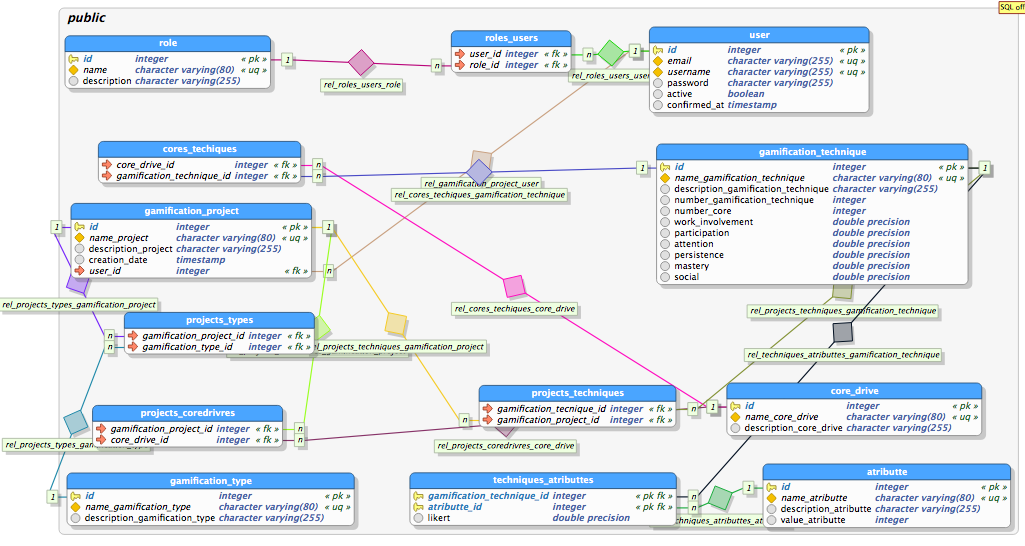
\includegraphics[keepaspectratio=true,scale=0.4]{figuras/gamifierdados.png}
	\caption{Modelo de dados do Gamifier.\label{fig06}}
\end{figure}

O banco contém atualmente treze tabelas, sendo que cinco delas são oriundas de relacionamentos n para n, o restante são as entidades que espelham as classes modelos da aplicação. 
As entidades principais do modelo são:

\begin{itemize}
\item  \textbf \textit{User:} Representa o usuário final da aplicação;
\item  \textbf \textit{Core drive:} Representa as unidades principais do  \textit{framework} Octalysis;
\item  \textbf \textit{Gamification project:} Representata os projetos de gamificação criados na ferramenta;
\item  \textbf \textit{Attribute:} Represeta os atributos selecionados para extender o octalysis;
\item  \textbf \textit{Gamification technique} Representa as técnicas de gamificação.
\item  \textbf \textit{Gamification type:} Representa o tipo de gamificação criado.
\end{itemize}

Os dados iniciais utilizados para a contrução da ferramenta são de extrema importância para o correto funcionamento da mesma. Sendo assim foram retirados da literatura, como no caso das unidades principais, técnicas de gamificação e atributos. Com um cuidado extra para a coleta das técnicas de gamificação, todas as técnicas presentes na aplicação foram extraídas do Funifier. A Fig.(\ref{fig07}) representa a tabela que contém as oito unidades principais.


\begin{figure}[h]
	\centering
		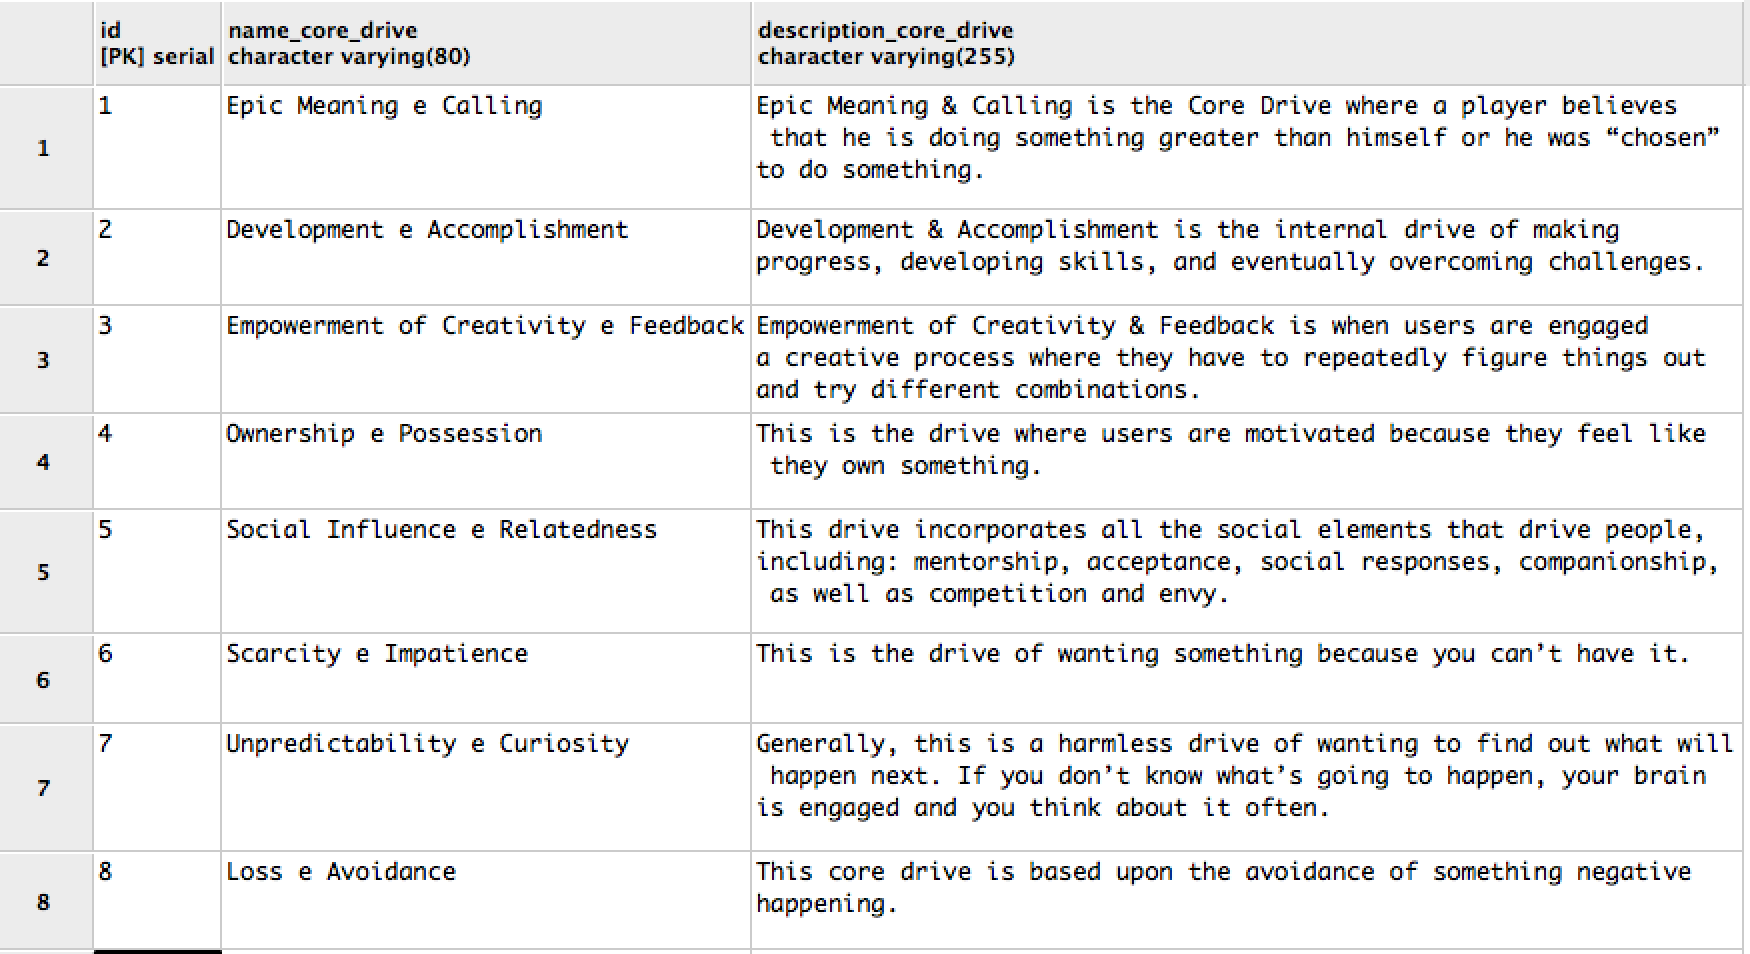
\includegraphics[keepaspectratio=true,scale=0.5]{figuras/mb.png}
	\caption{Exemplo de tabela presente na aplicação.\label{fig07}}
\end{figure}



\begin{figure}[h]
	\centering
		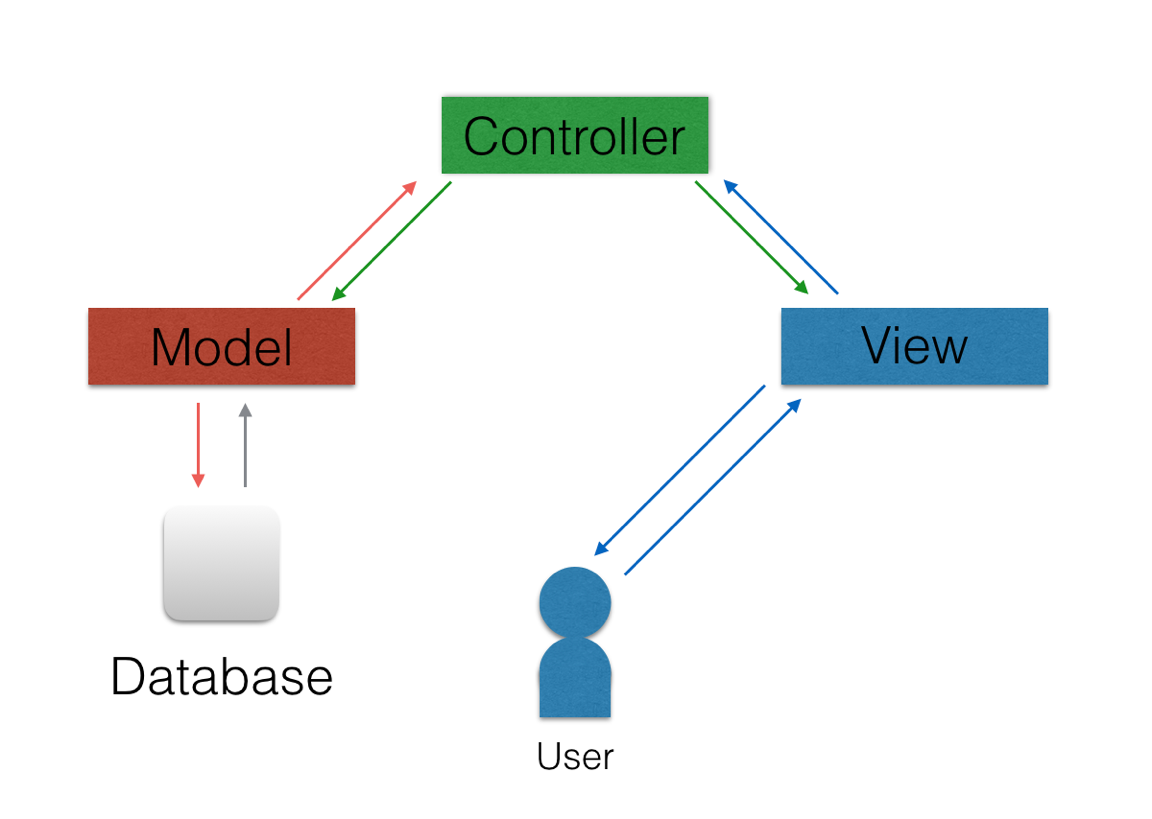
\includegraphics[keepaspectratio=true,scale=0.8]{figuras/MVC.png}
	\caption{Arquitetura MVC.\label{fig08}}
\end{figure}

O modelo arquitetural seguido para a construção da ferramenta foi o MVC. Segundo \cite{macoratti2009padroes} a abordagem da aquitetura MVC é composta por três objetos, o modelo, a visão e o controlador. O modelo é o objeto de aplicação, a visão é a apresentação da tela e o controlador é a maneira que define como a interface irá reagir as entradas do usuário.

 A  Fig.(\ref{fig08}) representa o MVC utilizado no projeto com a adição do usuário final. As setas representam a comunicação entre os módulos.\newpage
O banco de dados (\textit{database}) presente na figura representa o PostgreSQL e o SQLAlchemy. As modelos (\textit{Model}) e as controladoras (\textit{Controller}) foram contruídas em Python. A visão (\textit{View}) foi desenvolvida utilizando Jinja2 associada ao Bootstrap.

Diversos outros componentes foram necessários para dar vida ao Gamifier, desde de bibliotecas que foram importadas até máquinas virtuais e ferramentas de versionamento, as mais importantes foram destacadas nesta seção. 

\subsection {Desenvolvimento}

O Gamifier será desenvolvido para plataforma web, onde o usuário irá construir o projeto de gamificação a partir das técnicas de gamificação ou partir das unidades principais, o usuário terá a liberdade de escolher como iniciar o projeto. 

Para desenvolvimento da ferramenta prentende-se fazer uso do SCRUM com adaptações adequadas ao contexto do trabalho, será levantado o \textit{backlog} de produto, \textit{backlog} da \textit{sprint}, escrita de histórias, detalhamento em tarefas e definição de critérios de aceitação, \textit{sprints} com duração de duas semanas e retrospectiva ao fim das \textit{sprints}.



\subsubsection {Codificação}

O desenvolvimento iniciou-se com a construção das modelos e a criação do banco de dados, um exemplo das modelos podem ser visto na Fig.(\ref{fig09}). 


\begin{figure}[h]
	\centering
		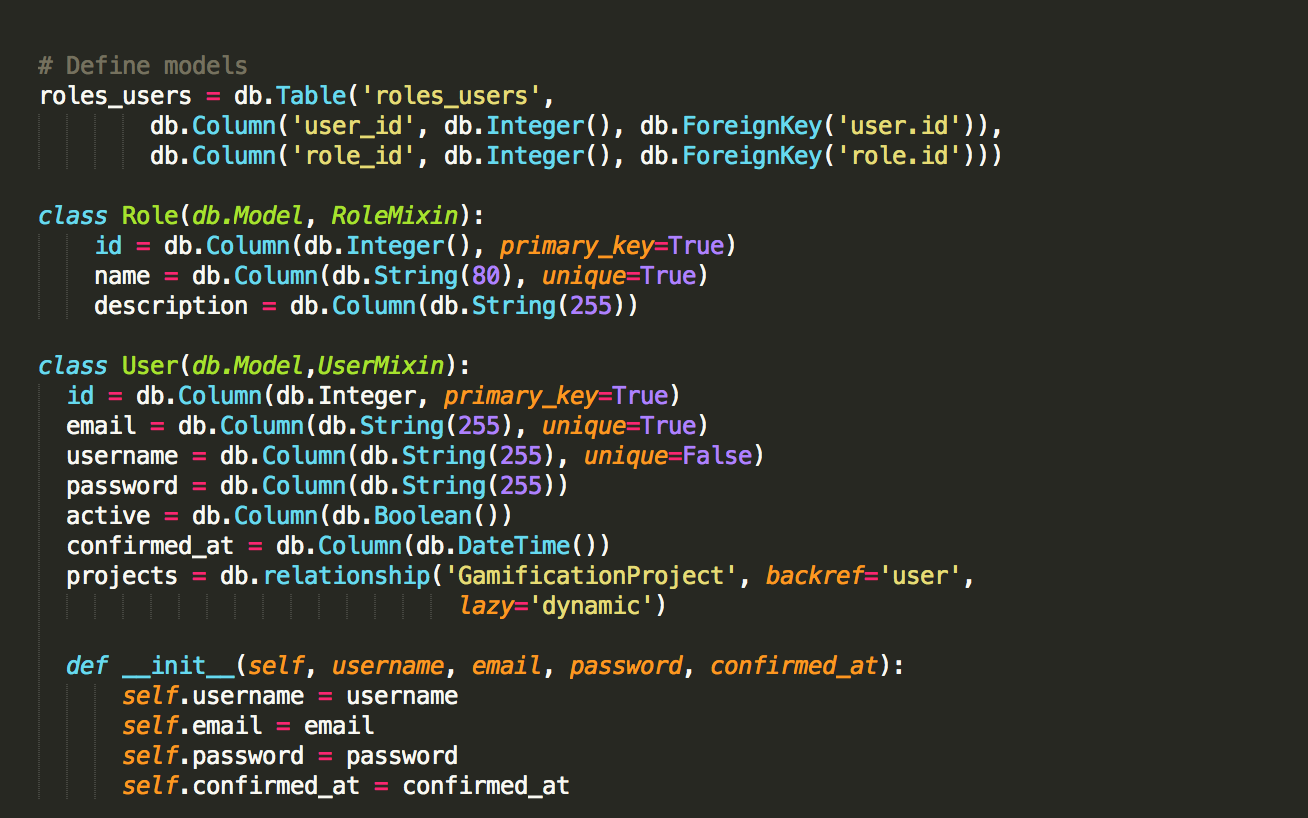
\includegraphics[keepaspectratio=true,scale=0.8]{figuras/modelo.png}
	\caption{Exemplo de classes modelos e relacionamento entre elas.\label{fig09}}
\end{figure}


Com a criação das modelos, o CRUD de usuário e projeto foram as primeiras tarefas a serem iniciadas. A Fig.(\ref{fig09}) exemplifica a classe de usuário, a classe de papeis desses usuários e o relacionamento entre elas. 

Na Fig.(\ref{fig09}) é possível notar ainda o relacionamento entre a classe \textit{User} e a classe \textit{GamificationProject} que corresponde aos projetos de gamificação. Cada usuário pode ter diversos projetos associados a si.


O uso do \textit{toolkit} SQLAlchemy  permite que as classes modelos criadas em Python gerem as entidades do banco de dados, sem que seja necessário a criação de um \textit{script} para tal. Os relacionamentos presentes na figura também são gerados de forma automática pelo \textit{toolkit}, que os reconhece e os insere corretamente de acordo com as peculiaridades de cada um.

Após concluída a etapa de criação das classes modelos e organização da arquitetura a tela de criação de projetos de gamificação começou a tomar forma. 


Com todas as técnicas e unidades principais cadastradas no banco de dados era possível criar projetos de gamificação simples. A Fig.(\ref{fig10}) representa a tela de criação de projetos do Gamifier.


\begin{figure}[h]
	\centering
		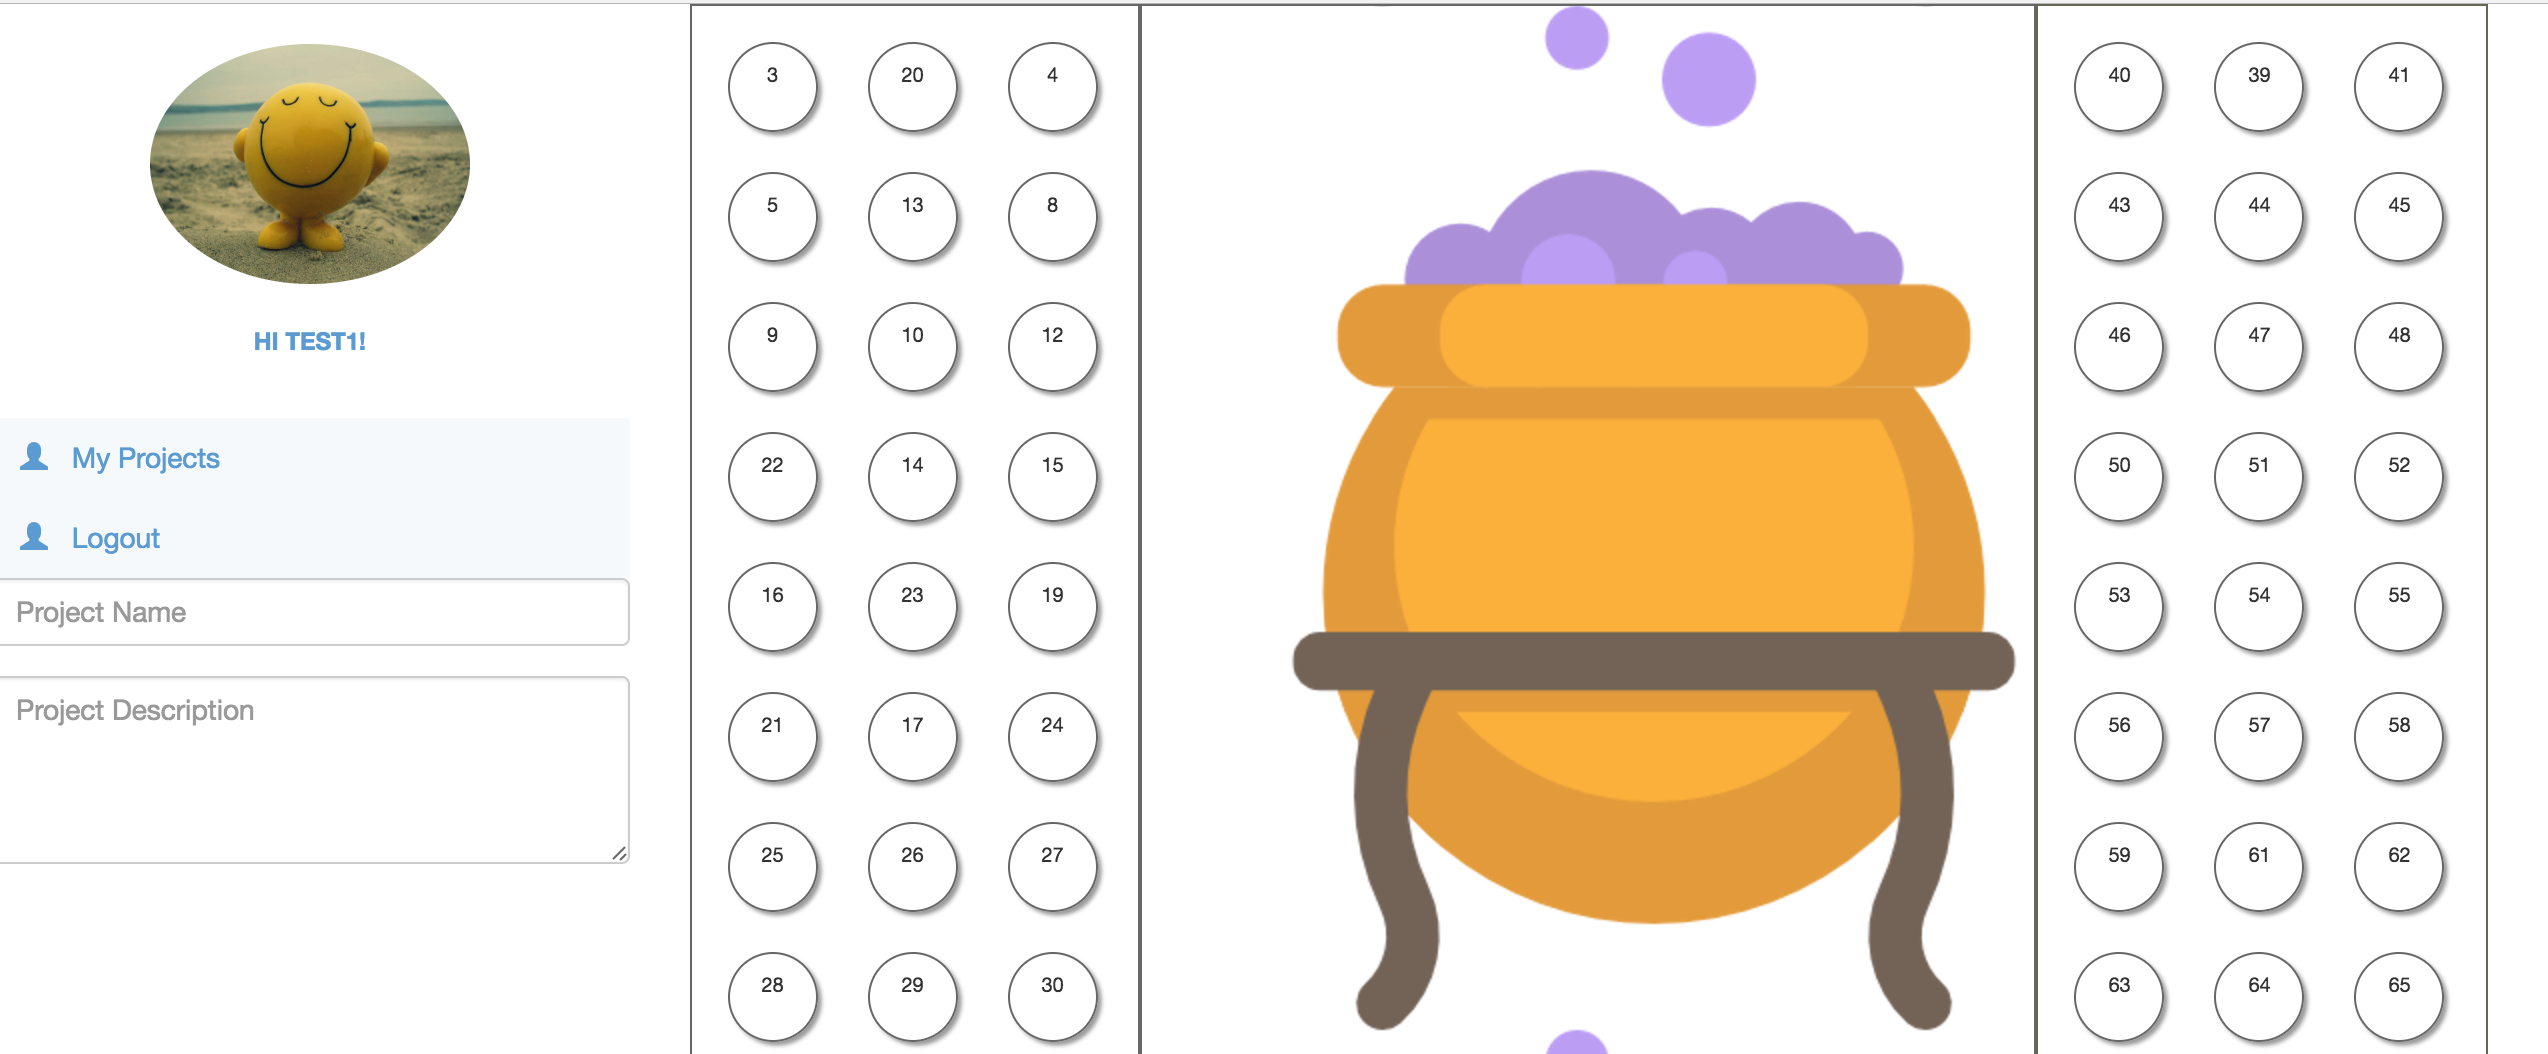
\includegraphics[keepaspectratio=true,scale=0.4]{figuras/telainicial.png}
	\caption{Tela de criação de projetos de gamificação.\label{fig10}}
\end{figure}


Cada círculo pequeno presente na Fig.(\ref{fig10}) representa uma técnica de gamificação, ao se passar o mouse em cada uma é possível obter informações sobre a mesma. Cria-se projetos de gamificação arrastando-se as técnicas desejadas pra dentro do \textit{container} ao centro, representado pelo caldeirão.

As técnicas representadas possuem os atributos caracterizadores, quando um projeto de gamificação está sendo criado os atributos associados as técnicas já estão presentes. Ao se escolher uma técnica pra fazer parte do projeto, os atributos também são indiretamente escolhidos.

O usuário pode arrastar e soltar técnicas de gamificação para fazer parte do projeto ou para deixar de fazer parte do projeto em qualquer momento da construção. 

O conjunto de técnicas de gamificação selecionadas representam o projeto de gamificação, o usuário pode dar um nome e uma descrição para cada um dos seus projetos. Cada usuário tem a possibilidade de construir inúmeros projetos e editá-los sempre que sentir necessidade.\newpage

Após finalizar a construção do projeto o usuário é direcionado para uma página com um \textit{feedback} do projeto que acabou de construir. A página é representada na Fig.(\ref{fig11}). 

\begin{figure}[h]
	\centering
		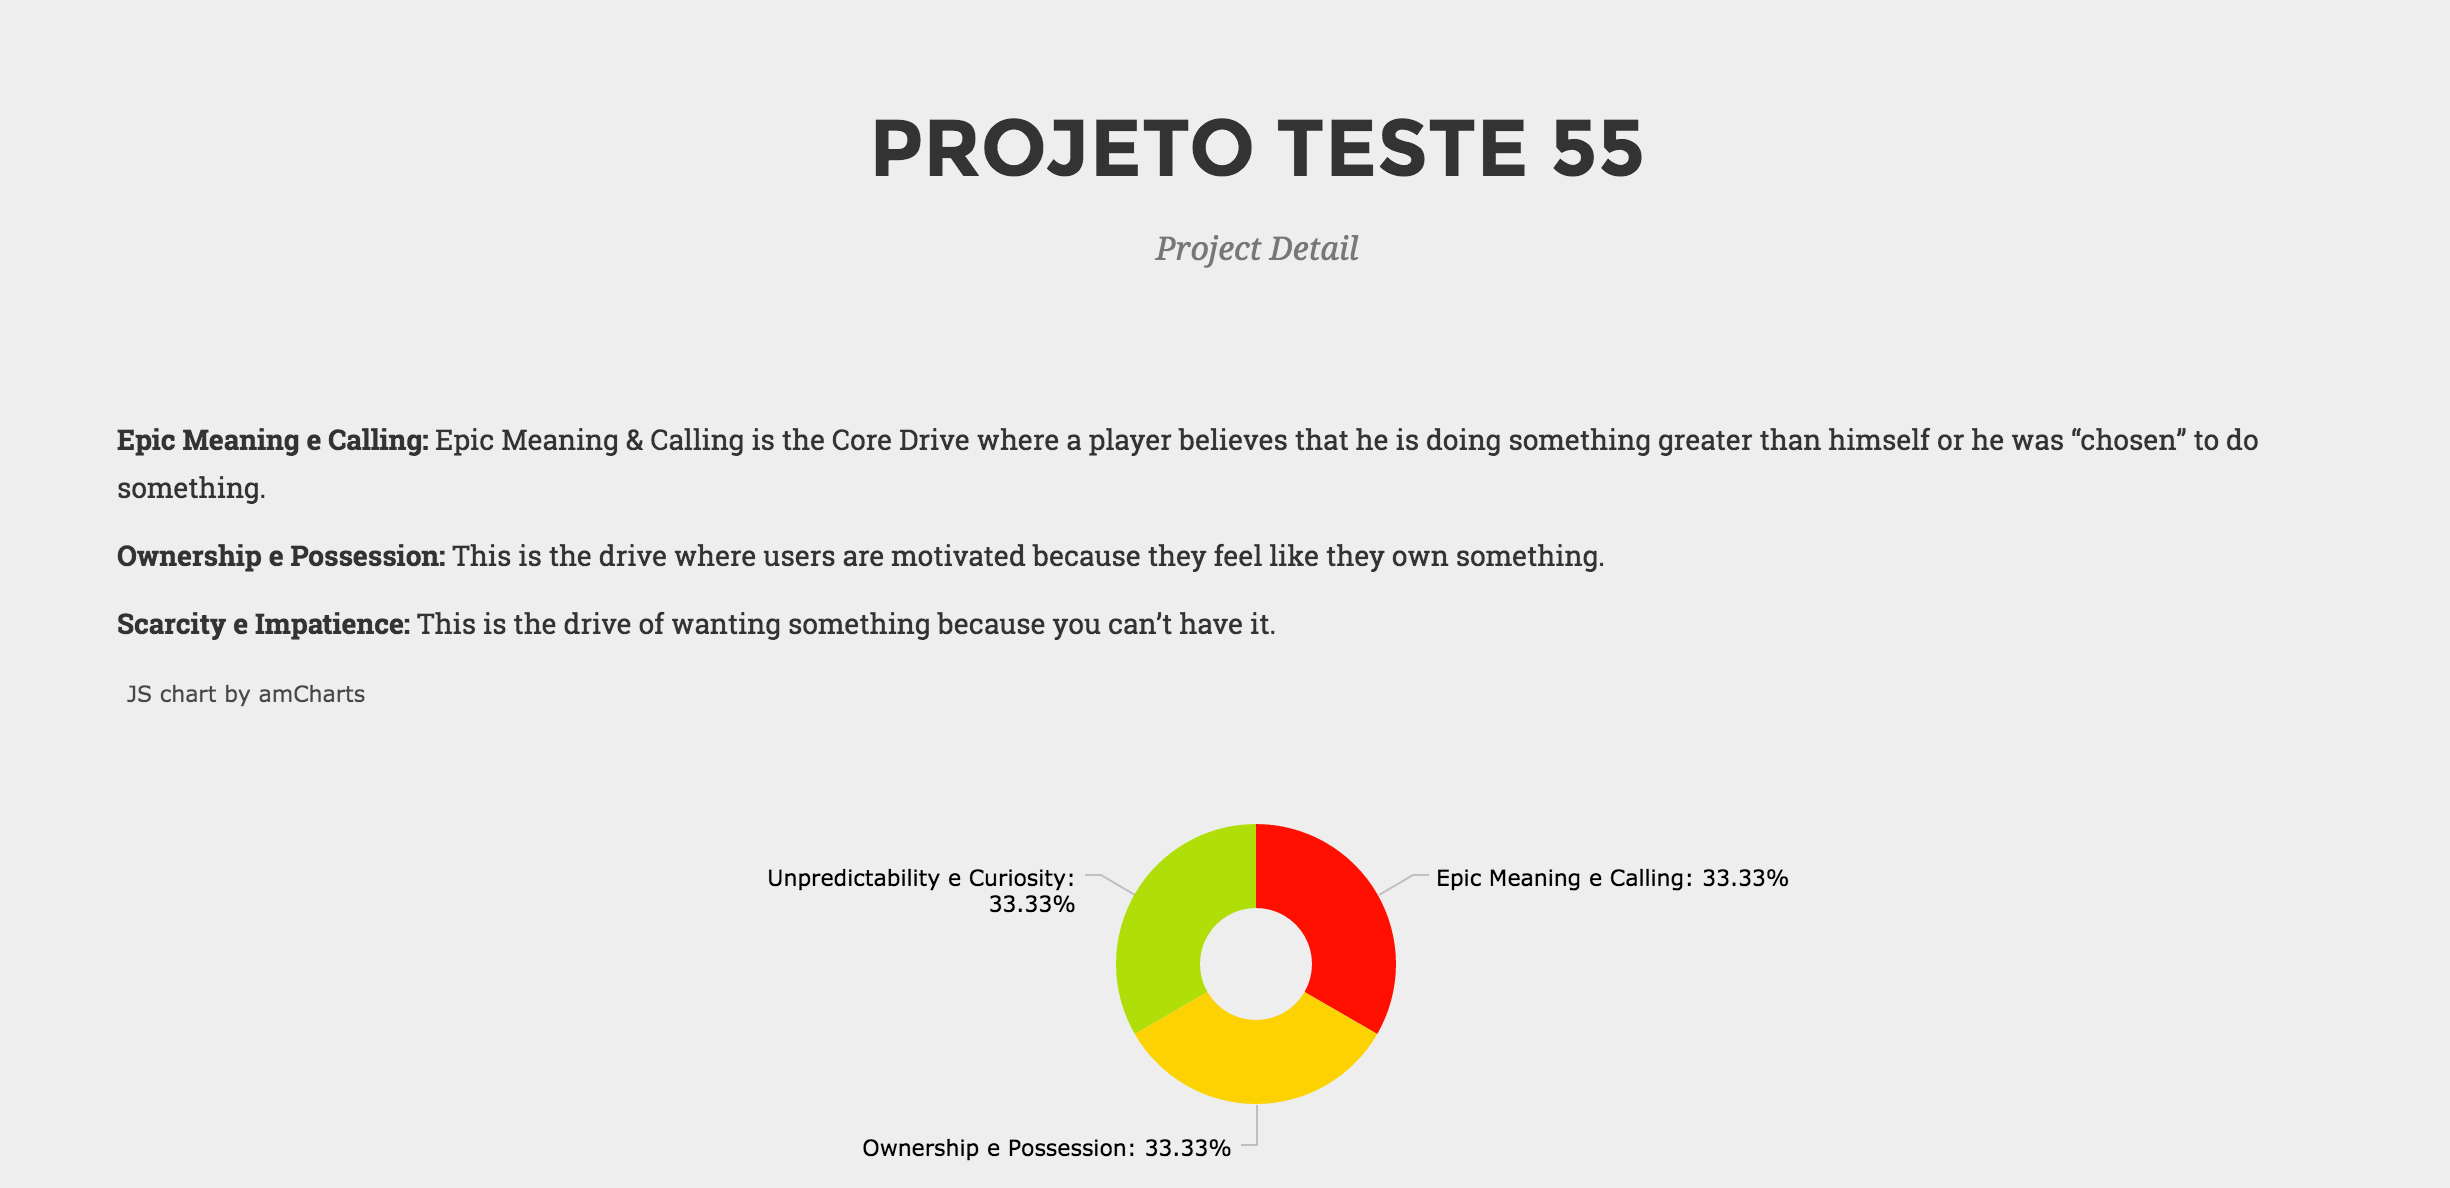
\includegraphics[keepaspectratio=true,scale=0.4]{figuras/detail.png}
	\caption{Tela de \textit{feedback} de projetos de gamificação, unidades principais.\label{fig11}}
\end{figure}


A página contém um gráfico que informa a porcentagem de cada unidade principal presente no projeto criado e a descrição de cada uma delas. O exemplo da Fig.(\ref{fig11}) contém a mesma proporção de três unidades principais, \textit{Epic Meaning and Calling}, \textit{Ownership and Possession} e \textit{Scarcity and Impatience}. 

Caso o projeto construído se enquadre dentro de um dos quatro tipos de gamificação (\textit{White Hat}, \textit{Black Hat}, \textit{Left Brain} ou \textit{Right Brain}) destacados por \cite{chou2015actionable}  além da descrição de cada unidade principal o usuário também será informado sobre o tipo de gamificação que construiu.


As unidades principais não utilizadas pelo usuário são omitidas. O cálculo de porcentagem de presença no projeto também exclui as UPs não utilizadas. A apresentação de dados aos usuários é feita sempre de maneira dinâmica. 

As requisições feitas ao banco de dados são as mínimas necessárias. Desta maneira todo o cálculo relacionado as técnicas e UPs é feito em tempo de execução utilizando \textit{javascript}. 

A  Fig.(\ref{fig12}) representa um dos métodos utilizados para a realização deste cálculo.\newpage

\begin{figure}[h]
	\centering
		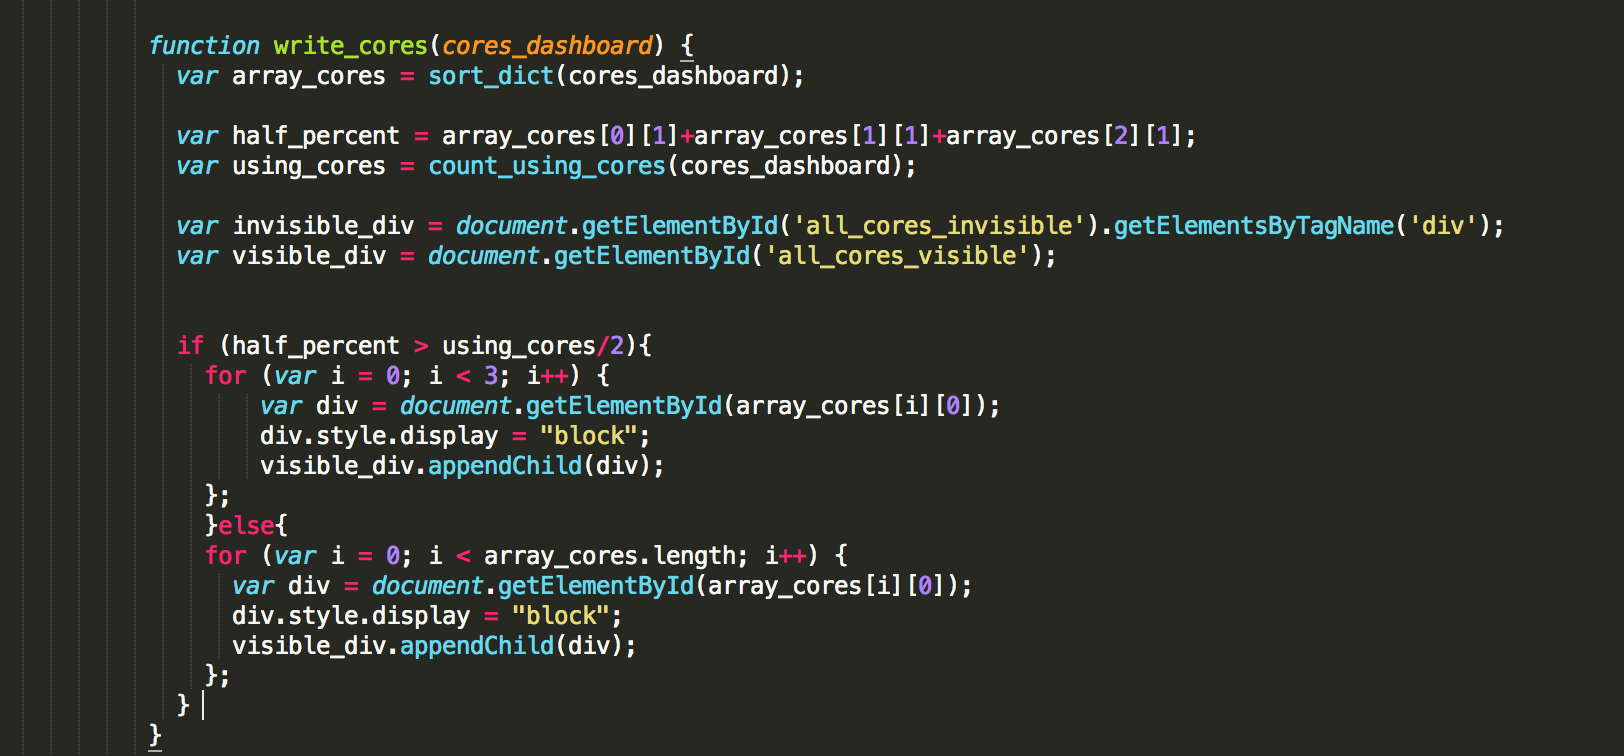
\includegraphics[keepaspectratio=true,scale=0.6]{figuras/cores.png}
	\caption{Método de cálculo de porcentagem dos cores.\label{fig12}}
\end{figure}

Um dos cálculos realizados verifica se do total de unidades principais utilizadas existem três unidades principais que representam mais que cinquenta porcento do projeto. Esse cálculo é feito assim que o usuário finaliza o projeto e o resultado influencia na seleção informações apresentadas na tela de \textit{feedback}. 

A tela de \textit{feedback} do projeto apresenta também a porcentagem que cada atributo representa no projeto construído. Todas as UPs são compostas por técnicas. Quando  uma técnica é selecionada para fazer parte do projeto os seis atributos que a compõe também são. 

Como dito anteriormente neste trabalho, os atributos recebem um valor que segue a escala de Likert, a escala utilizada varia de um a cinco.  Essa escala mensura o grau de pertencimento do atributo a técnica, quanto mais próximo de cinco o valor estiver, mais aquele atributo está presente na técnica e mais influência exerce sobre ela. 

Todas as técnicas presentes na ferramenta Gamifier tiveram seus atributos valorados. Três pessoas que tinham conhecimento sobre o \textit{Framework} Octalysis e seus componentes valoraram individualmente os atributos de cada uma das técnicas.

 O valor final que cada atributo associado a uma técnica recebeu corresponde a média entre os valores das três pessoas. O passo a passo realizado para efetuar essa valoração é ilustrado a seguir, na Fig. (\ref{fig12}).\newpage


\begin{figure}[h]
	\centering
		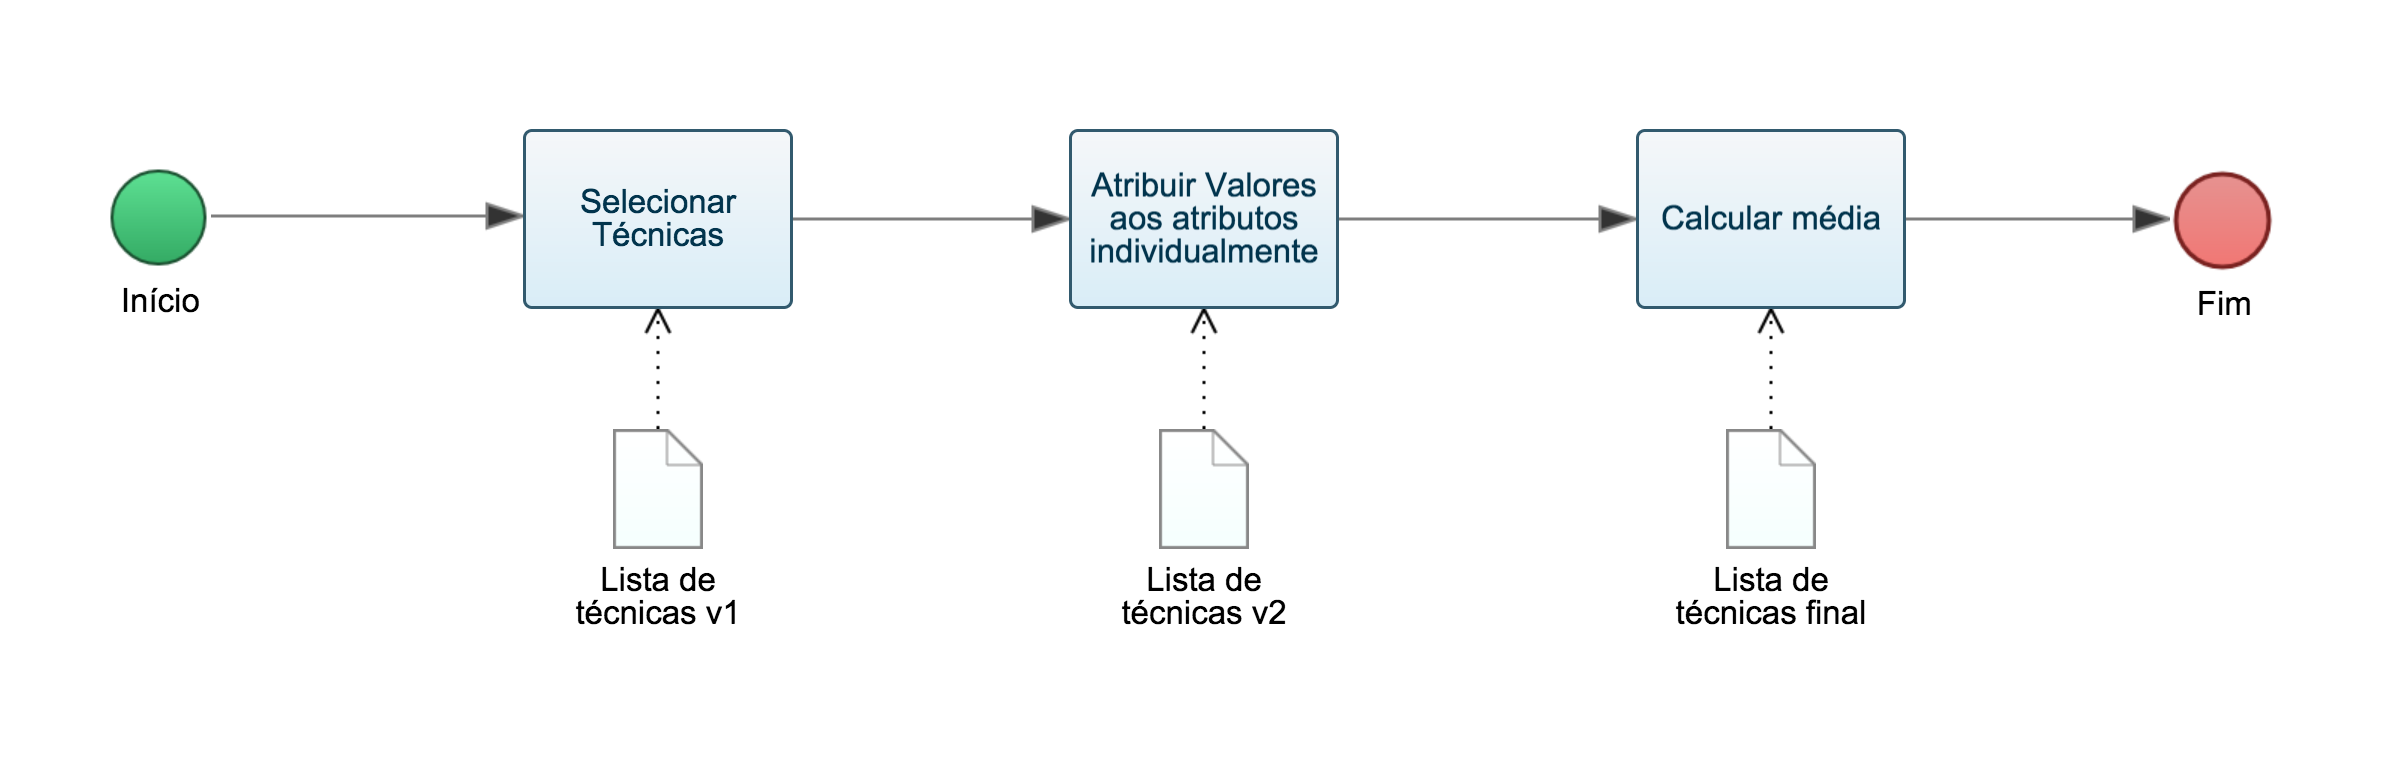
\includegraphics[keepaspectratio=true,scale=0.4]{figuras/fluxo.png}
	\caption{Fluxo de valoração dos atributos.\label{fig12}}
\end{figure}


\begin{itemize}
\item  \textbf {Selecionar Técnicas:} As técnicas de gamificação do Octalysis foram levantadas. O levantamento inicial foi feito nos livros e materiais do autor do \textit{framework} e consolidadas com o levantamento feito no Funifier.
\item  \textbf {Atribuir Valores aos Atributos:} Cada um dos responsáveis pela valoração dos atributos deu nota individualmente para todos os atributos. 
\item  \textbf {Calcular média:} A média dos três valores foi definida como falor final que cada atributo ;

\end{itemize}

Cada técnica possui os mesmos atributos, mas os atributos possuem valores diferentes de acordo com a técnica a qual pertecem. A tela de \textit{feedback} também apresenta o quão presente cada atributo está no projeto. 


A Fig.(\ref{fig13}) apresenta o gráfico dos atributos caracterizadores das técnicas de gamificação. É possível ver no gráfico de exemplo que o atributo envolvimento com o trabalho é o mais significante no projeto de gamificação em questão. A socialização vem em segundo lugar, seguida de participação, atenção, domínio e persistência.	


\begin{figure}[h]
	\centering
		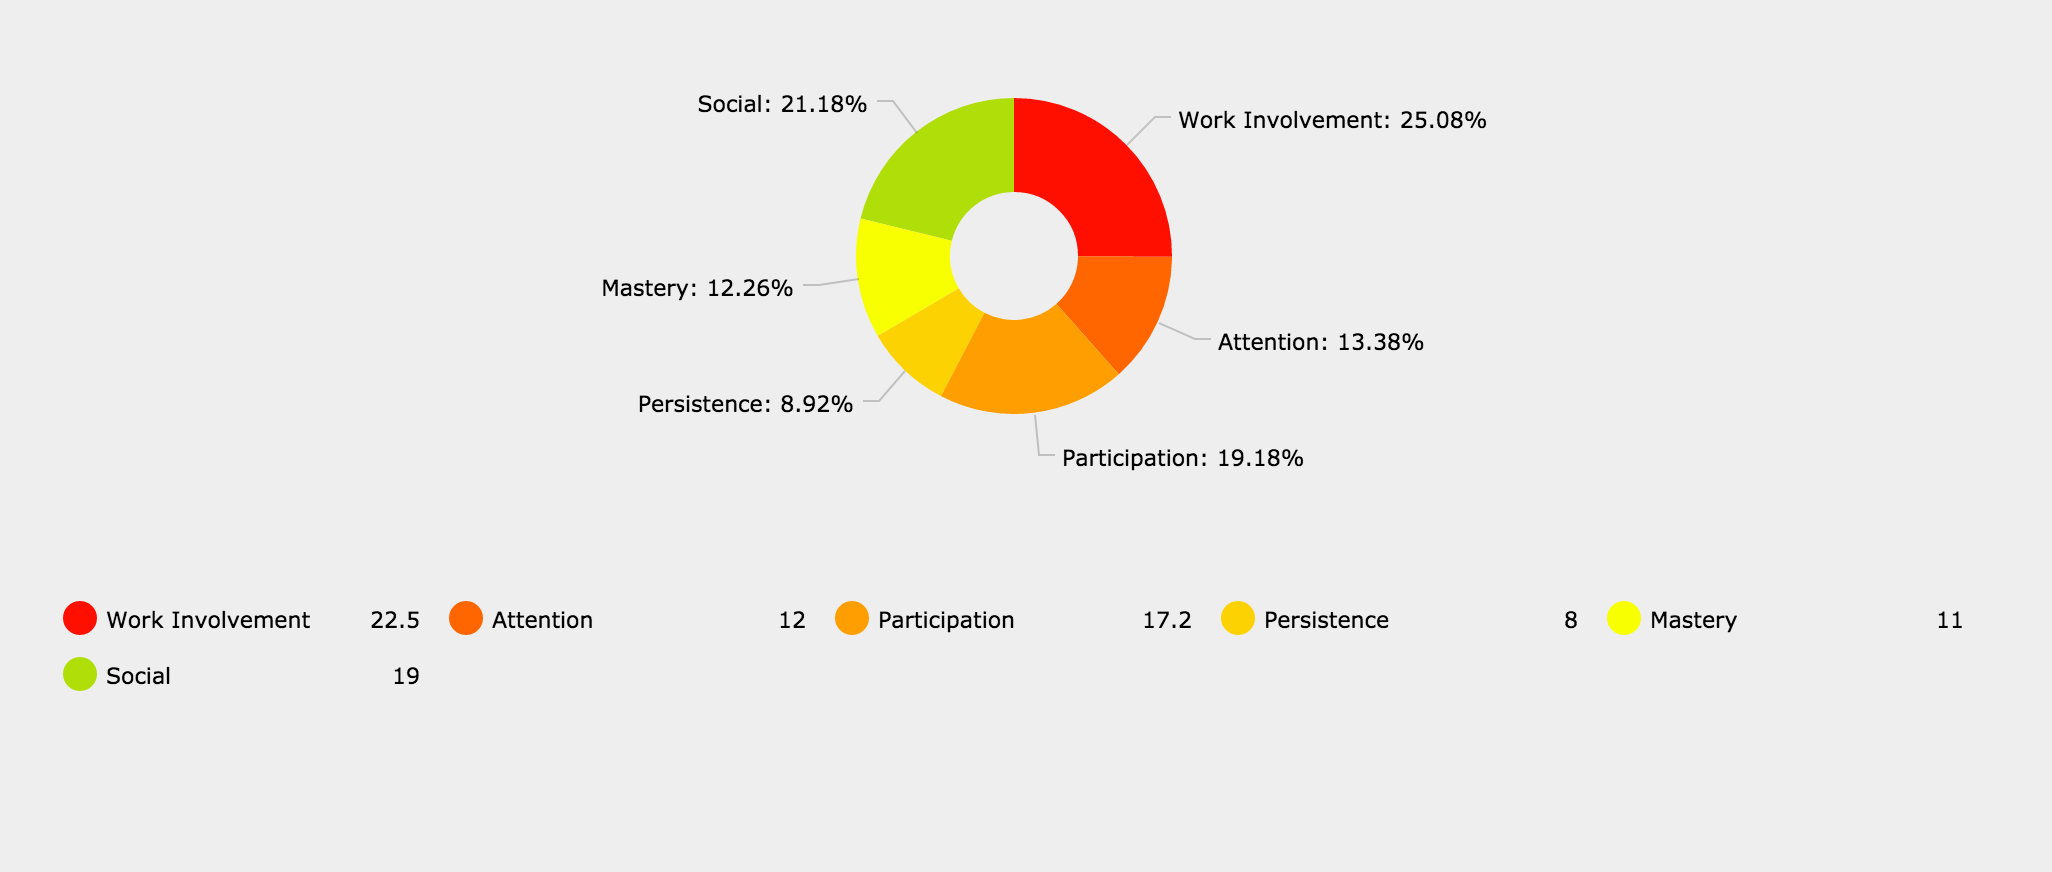
\includegraphics[keepaspectratio=true,scale=0.35]{figuras/atributos.png}
	\caption{Tela de \textit{feedback} de projetos de gamificação, atributos..\label{fig13}}
\end{figure}

Os mesmos valores utilizados neste trabalho também foram empregados para a construção do artigo Metodologia para avaliação da gamificação em jogos, publicado no Simpósio Brasileiro de Informática na Educação (SBIE) de 2016. O cálculo para verificar a influência do atributo ao projeto no entanto, não é o mesmo utilizado no artigo, apesar de fazer uso dos mesmos dados.


O cálculo de presença dos atributos é feito através de uma soma simples. Por exemplo, se um projeto contém vinte e duas técnicas o atributo envolvimento com o trabalho também aparece vinte e duas vezes, afinal ele está presente em todas elas. 

Para cada técnica o atributo recebeu um valor e a soma desses valores representa a porcentagem de influência desse atributo ao projeto. Quanto mais alto o valor, mais influência. O método que realiza este cálculo por ser visto na Fig. (\ref{fig14}).


\begin{figure}[h]
	\centering
		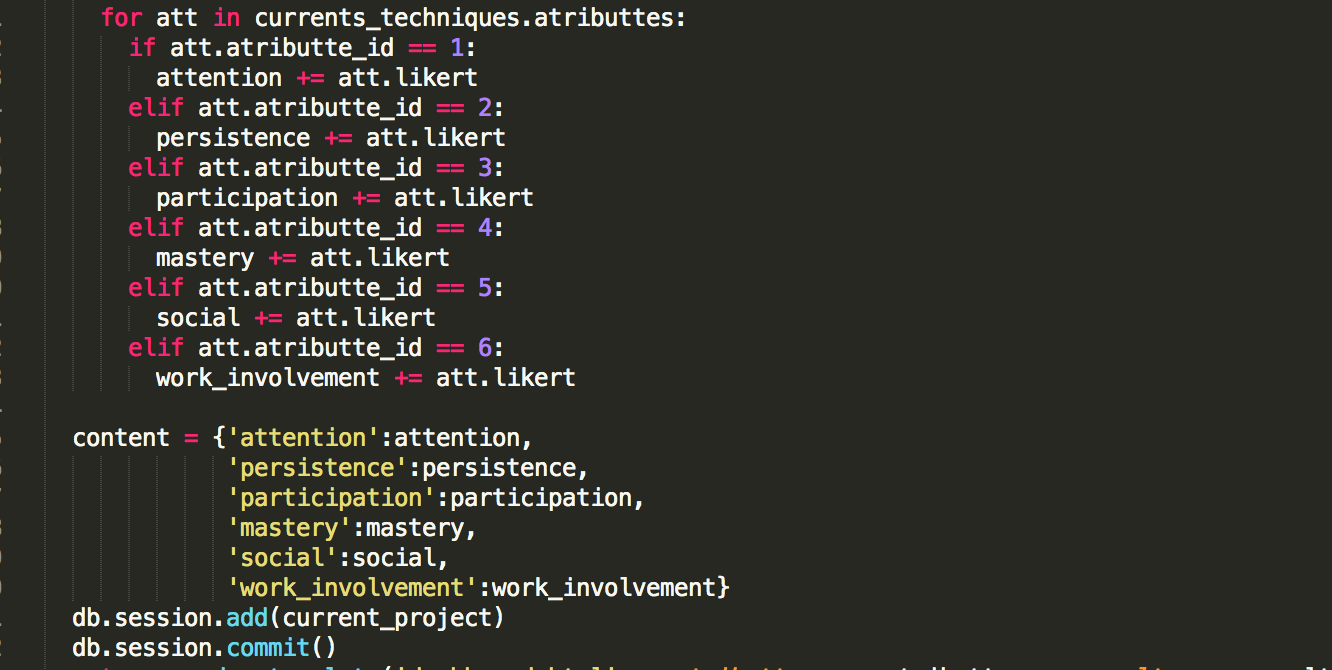
\includegraphics[keepaspectratio=true,scale=0.6]{figuras/att.png}
	\caption{Método de cálculo de porcentagem dos atributos.\label{fig14}}
\end{figure}


Para realizar o cálculo percorre-se o vetor de técnicas, mas apenas as técnicas presentes no projeto recém criado. Enquanto as técnicas são percorridas os valores dos atributos são somados. Um dicionário de atributos é criado, associando cada atributo com o valor total da sua soma.

 O projeto é adicionado ao banco, com todas as unidades principais, técnicas a tributos relacionados a ele. O dicionário é enviado para a camada de visão e é apresentado ao usuário na forma do gráfico visto na  Fig.(\ref{fig13}).

No momento que o usuário finaliza o projeto e é redirecionado para a página de \textit{feedback} o projeto é salvo no banco de dados. Caso o usuário tenha interesse ele pode exportar o seu projeto em formato de tabela com a extensão CSV. A tabela exportada contém todas as UPs utilizadas no projeto, as técnicas, seus respectivos números, data de criação, nome e descrição do projeto. Uma tabela exemplo está presente no primeiro apendice deste trabalho.

Caso o usuário queira ter acesso ao conteúdo da página de \textit{feedback} após encerrar um projeto ele pode visualizar em forma de relatório ou gerar um aquivo com as informações do projeto com a extensão PDF. O usuário não pode modificar o resultado do projeto, caso ele queira fazer alguma alteração ele deverá alterar o projeto original e gerar um relatório a partir das modificações. Um exemplo do relatório gerado está contido no segundo apendice deste trabalho.

